Problem number 3 required a hierarchical implementation of the actions.
We decided to construct it as described in the diagram \ref{Actions diagram}
\begin{figure}[h!]
    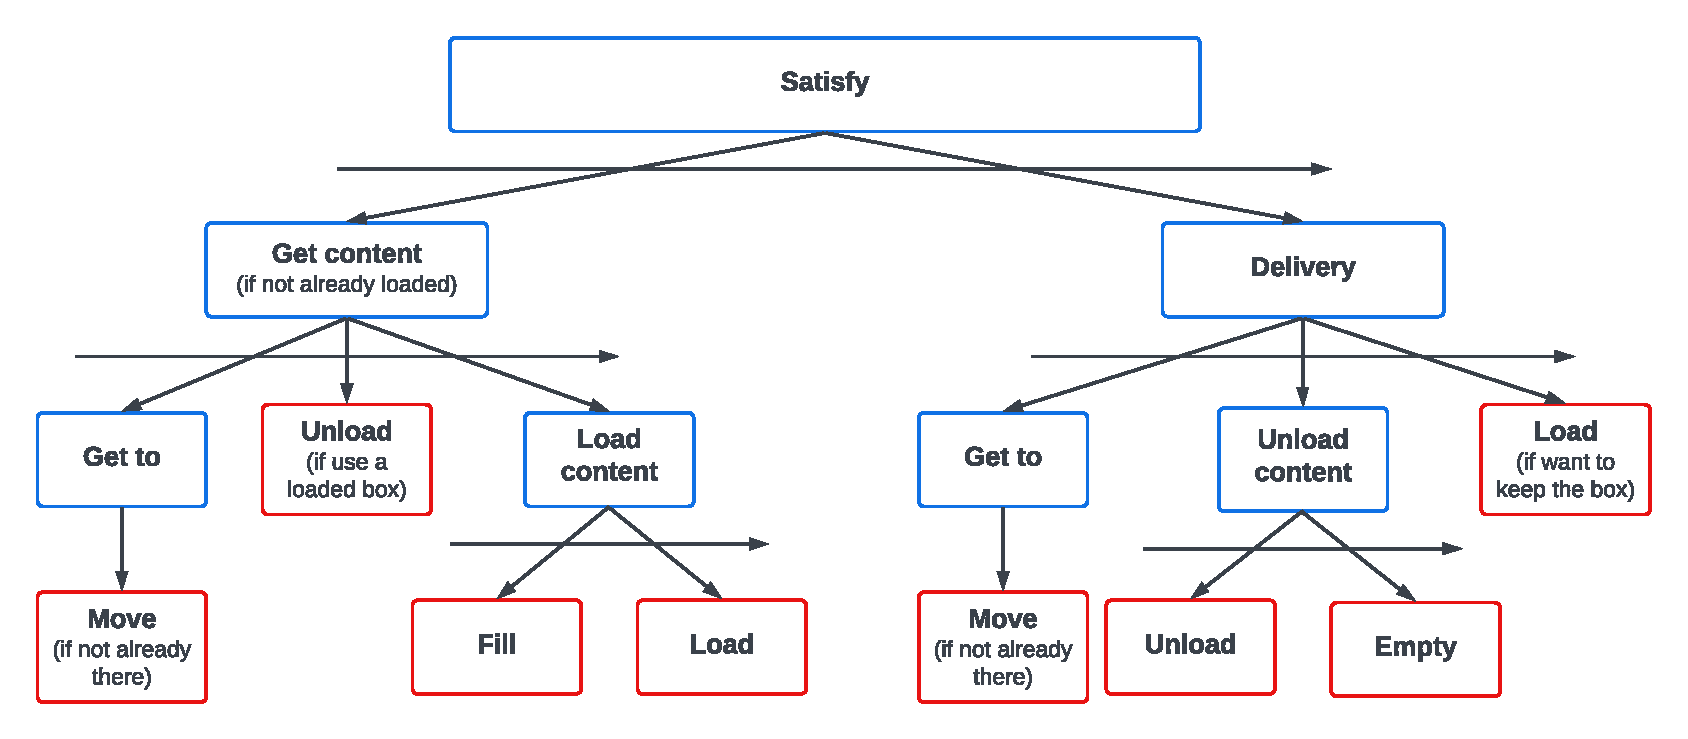
\includegraphics[scale = 0.35]{images/Actions_diagram.pdf}
    \label{Actions diagram}
\end{figure}
The main task is to \textbf{satisfy} a person delivering to him/her a specific supply.
To do that the robot first has to \textbf{get the content}, then to \textbf{delivery} it.
To \textbf{get the content} the robot \textbf{gets to} the place where the supply is stored, and \textbf{loads} it on the carrier (\textbf{fill} + \textbf{load}).
The \textbf{delivery} consists of \textbf{get to} the place where the person is and \textbf{unload the content} (\textbf{unload} + \textbf{empty}).
This is a standard workflow, of which there are some variations listed here:
\begin{itemize}
    \item A robot could already have the needed supply in a box it is carrying. For this we have an alternative method for the \textbf{get\_content} task, which is \textbf{m\_already\_got\_content} that is implemented by the action \textbf{no\_load}, which basically does nothing.
    \item A robot could already be where it has to go, so the \textbf{get\_to} task is also implemented using the \textbf{m\_already\_there} method that calls the \textbf{no\_move} action.
    \item In case the number of boxes is less than the number of people to satisfy, A robot must keep the box after delivering the supplies, to do that there are 2 implementations for the \textbf{delivery} action, one that \textbf{load} the box on the carrier after it empties it and one that does not.
    \item When a robot wants to re-use a box, it needs to \textbf{get\_content} using a box it is already in the carrier, for this reason there are 2 implementations of the \textbf{get\_content} task, one \textbf{unload} a box from the carrier before filling it and load it, the other does not.
\end{itemize} 
To test it we kept the same environment as in problem 2, with 7 \textbf{satisfy} tasks to perform.
We had to specify an ordering to keep the searching space sufficiently small and to find a plan in little time, if no temporal constraints are put, the ordering can be removed.